\documentclass[12pt]{article}

% Packages
\usepackage{geometry}
\usepackage{setspace}
\usepackage{xcolor}
\usepackage{enumitem}
\usepackage{graphicx}
\usepackage{listings}
\usepackage{xcolor}
\usepackage{changepage}
\usepackage{endnotes}
\usepackage{amsmath, amsthm, amsfonts, amssymb}

% Custom colors for code highlighting
\definecolor{codegreen}{rgb}{0,0.6,0}
\definecolor{codegray}{rgb}{0.5,0.5,0.5}
\definecolor{codepurple}{rgb}{0.58,0,0.82}
\definecolor{backcolour}{rgb}{0.95,0.95,0.92}

% Style for Python code
\lstset{
    language=Python,
    backgroundcolor=\color{backcolour},
    commentstyle=\color{codegreen},
    keywordstyle=\color{magenta},
    numberstyle=\tiny\color{codegray},
    stringstyle=\color{codepurple},
    basicstyle=\ttfamily\scriptsize,
    breakatwhitespace=false,
    breaklines=true,
    captionpos=b,
    keepspaces=true,
    numbers=left,
    numbersep=5pt,
    showspaces=false,
    showstringspaces=false,
    showtabs=false,
    tabsize=2
}

% Define theorem, definition, and proof environments
\newtheorem{theorem}{Theorem}
\newtheorem{definition}{Definition}
\newtheorem{lemma}{Lemma}
\newtheorem{corollary}{Corollary}
\newtheorem{proposition}{Proposition}
\newtheorem{example}{Example}
\newtheorem{remark}{Remark}

% Set up the page margins
\geometry{left=0.5in,right=0.5in,top=0.5in,bottom=0.75in}

\begin{document}
\doublespacing % Use this command for double spacing

\title{HW-08}
\author{Abraham J. Reines}
\date{\today}
\maketitle

\section{Introduction}
This section presents a detailed analysis of the relation \( R \) defined on the set \( A = \{ 0, 1, 2, 3 \} \). The relation \( R \) is given by \( R = \{ (1,2), (2,1), (1,3), (3,1) \} \).

\subsection{Graphical Representation of R}
The directed graph of the relation \( R \) is shown in Figure 1.

\begin{figure}[h]
    \centering
    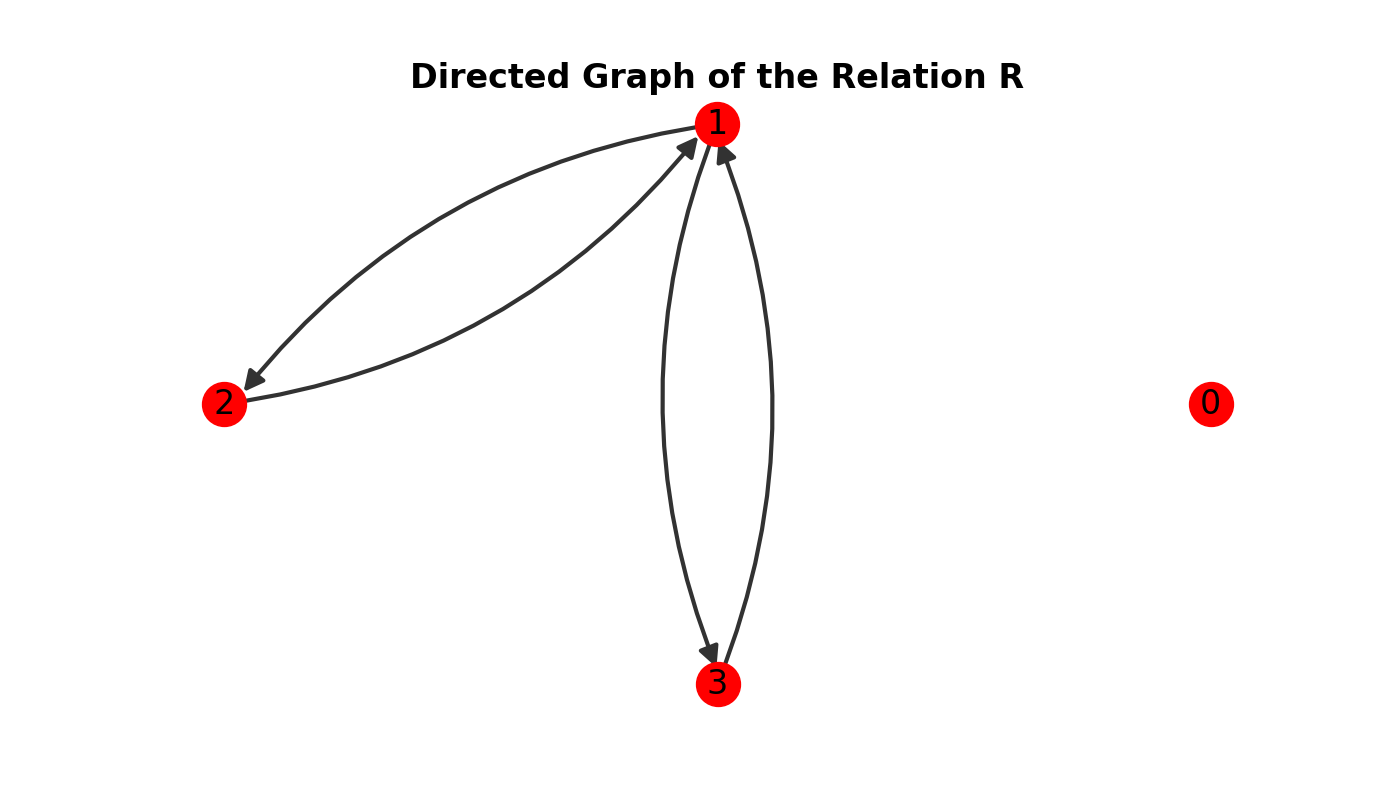
\includegraphics[width=0.75\textwidth]{Figure2.png} 
    \caption{Directed Graph of the Relation \( R \)}
    \label{fig:graphR}
\end{figure}

\subsection{Code for Figure 1:} To show logic behind the formulation of the Directed Graph.
\begin{lstlisting}
import matplotlib.pyplot as plt
import networkx as nx
from matplotlib.patches import FancyArrowPatch
from matplotlib.colors import LinearSegmentedColormap

class DirectedGraphVisualizer:
    """Visualizes a directed graph with arrow styling."""
    def __init__(self, nodes, edges):
        """Initialize the DirectedGraphVisualizer with nodes and edges."""
        self.graph = nx.DiGraph()
        self.graph.add_nodes_from(nodes)
        self.graph.add_edges_from(edges)

    def create_gradient_arrow(self, start_point, end_point, rad=0.5, arrowstyle='-|>', lw=2, mutation_scale=20):
        """Create a gradient colored arrow."""
        cmap = LinearSegmentedColormap.from_list("", ["black", "white", "yellow"])
        arrow = FancyArrowPatch(start_point, end_point, connectionstyle=f"arc3,rad={rad}",
                                arrowstyle=arrowstyle, lw=lw, mutation_scale=mutation_scale, 
                                color=cmap(0.1), linestyle='-', zorder=1)
        return arrow

    def draw_curved_edges(self, pos, ax, rad=0.2, arrowstyle='-|>', lw=3, mutation_scale=30):
        """Draw curved edges with gradient arrows."""
        for (u, v) in self.graph.edges():
            if (v, u) in self.graph.edges() and u < v:
                arrow = self.create_gradient_arrow(pos[u], pos[v], rad, arrowstyle, lw, mutation_scale)
                ax.add_patch(arrow)
                arrow = self.create_gradient_arrow(pos[v], pos[u], rad, arrowstyle, lw, mutation_scale)
                ax.add_patch(arrow)
            elif not (v, u) in self.graph.edges():
                arrow = self.create_gradient_arrow(pos[u], pos[v], 0, arrowstyle, lw, mutation_scale)
                ax.add_patch(arrow)

    def draw_graph(self, layout=nx.circular_layout, node_size=500, node_color="red", font_size=18, font_color="black"):
        """Draw the graph with arrows and nodes."""
        plt.figure(figsize=(8, 8))
        pos = layout(self.graph)
        ax = plt.gca()

        nx.draw_networkx_nodes(self.graph, pos, node_size=node_size, node_color=node_color, ax=ax)
        nx.draw_networkx_labels(self.graph, pos, font_size=font_size, font_color=font_color, ax=ax)
        self.draw_curved_edges(pos, ax)

        plt.title("Directed Graph of the Relation R", fontsize=18, fontweight='bold')
        plt.axis('off')
        plt.show()


A = {0, 1, 2, 3}
R = {(1, 2), (2, 1), (1, 3), (3, 1)}

graph_visualizer = DirectedGraphVisualizer(A, R)
graph_visualizer.draw_graph()
\end{lstlisting}

\subsection{Reflexivity and Irreflexivity}
\begin{theorem}
The relation \( R \) is irreflexive.
\end{theorem}
\begin{proof}
\begin{itemize}
    \item \textbf{Reflexive} if \(\forall a \in A, (a, a) \in R\).
    \item \textbf{Irreflexive} if \(\forall a \in A, (a, a) \notin R\).
    \item \textbf{Analysis}: Given no element in \( A \) is related to itself in \( R \), \( R \) is irreflexive.
    \item \textbf{Evidence for Irreflexivity}: None of the pairs \( (0,0) \), \( (1,1) \), \( (2,2) \), or \( (3,3) \) are in \( R \), confirming its irreflexivity.
    \item \textbf{Counterexample for Reflexivity}: Consider the element \( 0 \) in \( A \). Reflexivity requires \( (0,0) \) to be in \( R \). However, \( (0,0) \notin R \), thus \( R \) is not reflexive.
\end{itemize}
\end{proof}

\subsection{Symmetry and Asymmetry}
\begin{theorem}
The relation \( R \) is symmetric.
\end{theorem}
\begin{proof}
\begin{itemize}
    \item \textbf{Symmetric} if \(\forall (a, b) \in R, (b, a) \in R\).
    \item \textbf{Asymmetric} if \(\forall (a, b) \in R, (b, a) \notin R\).
    \item \textbf{Analysis}: Since for every pair \((a, b) \in R\), the pair \((b, a)\) is also in \( R \), the relation \( R \) is symmetric.
    \item \textbf{Evidence for Symmetry}: Pairs like \( (1,2) \) and \( (2,1) \), \( (1,3) \) and \( (3,1) \) are in \( R \), demonstrating its symmetry.
    \item \textbf{Counterexample for Asymmetry}: The pair \( (1,2) \) is in \( R \). For \( R \) to be asymmetric, \( (2,1) \) must not be in \( R \). However, \( (2,1) \in R \), violating asymmetry.
\end{itemize}
\end{proof}

\subsection{Transitivity}
\begin{theorem}
The relation \( R \) is not transitive.
\end{theorem}
\begin{proof}
\begin{itemize}
    \item \textbf{Transitive} if \(\forall (a, b), (b, c) \in R, (a, c) \in R\).
    \item \textbf{Analysis}: \( R \) is not transitive since there are no instances where \((a, b)\) and \((b, c)\) being in \( R \) lead to \((a, c)\) also being in \( R \).
    \item \textbf{Counterexample for Transitivity}: The pairs \( (1,2) \) and \( (2,1) \) are in \( R \). Transitivity requires \( (1,1) \) be in \( R \) as well. However, \( (1,1) \notin R \), indicating \( R \) is not transitive.
\end{itemize}
\end{proof}

\subsection{Code for Validating each property} To show logic behind the determination of each property.
\begin{lstlisting}
# Set A and relation R
A = {0, 1, 2, 3}
R = {(1, 2), (2, 1), (1, 3), (3, 1)}

# Function to check reflexivity
def is_reflexive(A, R):
    return all((a, a) in R for a in A)

# Function to check irreflexivity
def is_irreflexive(A, R):
    return all((a, a) not in R for a in A)

# Function to check symmetry
def is_symmetric(R):
    return all((b, a) in R for a, b in R)

# Function to check asymmetry
def is_asymmetric(R):
    return all((b, a) not in R for a, b in R)

# Function to check transitivity
def is_transitive(R):
    return all((a, c) in R for a, b in R for c in A if (a, b) in R and (b, c) in R)

# Validating each property
reflexivity = is_reflexive(A, R)
irreflexivity = is_irreflexive(A, R)
symmetry = is_symmetric(R)
asymmetry = is_asymmetric(R)
transitivity = is_transitive(R)

print(reflexivity, irreflexivity, symmetry, asymmetry, transitivity)
# Results: False True True False False
\end{lstlisting}

\subsection{Conclusion}
The comprehensive examination of the relation \( R \) defined on the set \( A = \{ 0, 1, 2, 3 \} \) elucidates several critical aspects of its character. Firstly, \( R \) is irreflexive, as demonstrated by the absence of self-pairs such as \( (0,0) \) in \( R \). This observation is pivotal, underscoring no element in \( A \) is related to itself under \( R \).

Furthermore, the analysis firmly establishes \( R \) is symmetric. This conclusion is drawn from the observation for every pair \( (a, b) \) in \( R \), the reciprocal pair \( (b, a) \) is also found within \( R \), a hallmark of symmetric relations. The pairs \( (1,2) \) and \( (2,1) \), along with \( (1,3) \) and \( (3,1) \), are testament to this symmetric nature.

However, when it comes to transitivity, \( R \) does not fulfill the necessary criteria. The absence of certain consequential pairs, such as \( (1,1) \) despite the presence of \( (1,2) \) and \( (2,1) \) in \( R \), clearly illustrates this shortfall. Thus, \( R \) is not a transitive relation.

In summary, the relation \( R \) on the set \( A \) is irreflexive and symmetric but not transitive. The detailed counterexamples provided for each property not only highlight where \( R \) diverges from these specific relational properties but also enrich our understanding of the nature of relations in discrete mathematics.

% QUESTION TWO

\section{Introduction}
In the realm of discrete mathematics, the concept of transitive closure plays a crucial role in understanding the properties of binary relations. 

\begin{definition}[Binary Relation]
A \textbf{binary relation} \( R \) on a set \( A \) is a collection of ordered pairs of elements from \( A \). The relation is said to be \textit{transitive} if whenever an element \( a \) is related to \( b \), and \( b \) is related to \( c \), then \( a \) is also related to \( c \).
\end{definition}

\begin{definition}[Transitive Closure]
The \textbf{transitive closure} of a binary relation \( R \), denoted as \( R^t \), is the smallest transitive relation on \( A \) which contains all the pairs in \( R \).
\end{definition}

\subsection{Example and Computation}

\begin{example}
Consider the set \( A = \{ 0, 1, 2, 3 \} \) and the binary relation \( T = \{ (0, 2), (1, 0), (2, 3), (3, 1) \} \) defined on \( A \). Our objective is to find the transitive closure \( T^t \) of \( T \).
\end{example}

\begin{proposition}
The transitive closure \( T^t \) of the relation \( T \) is obtained by adding the least number of ordered pairs to \( T \) to ensure transitivity, making \( T^t \) the smallest transitive relation containing \( T \). It is important to note \( T \subseteq T^t \).
\end{proposition}

\begin{proof}
A relation fails to be transitive when it fails to contain certain ordered pairs. For example, if \( (1, 3) \) and \( (3, 4) \) are in a relation \( R \), then the pair \( (1, 4) \) must be in \( R \) for \( R \) to be transitive. To obtain a transitive relation from one which is not transitive, it is necessary to add the missing ordered pairs.

To compute the transitive closure \( T^t \) of \( T \), we follow these steps:

1. Identify all pairs \((x, z)\) such that there exists a \( y \) in \( A \) where \( (x, y) \) and \( (y, z) \) are in \( T \). For instance, since \( (0, 2) \) and \( (2, 3) \) are in \( T \), the pair \( (0, 3) \) must be included in \( T^t \) for transitivity.

2. Add these identified pairs to \( T \) to form \( T^t \), ensuring \( T \subseteq T^t \).

Applying this method to \( T \), the transitive closure \( T^t \) is:
\[ T^t = \{ (0, 0), (0, 1), (0, 2), (0, 3), (1, 0), (1, 1), (1, 2), (1, 3), (2, 0), (2, 1), (2, 2), (2, 3), (3, 0), (3, 1), (3, 2), (3, 3) \} \]
This includes all possible pairs for \( A \), thus fulfilling the criteria for transitivity and confirming \( T \subseteq T^t \).
\end{proof}

\subsection{Code for Validating transitive closure of T} To show logic behind the determination of transitive closure.
\begin{lstlisting}
from itertools import product

# The original relation T
T = {(0, 2), (1, 0), (2, 3), (3, 1)}

# Function to compute the transitive closure
def transitive_closure(rel):
    closure = set(rel)
    while True:
        new_relations = {(x, w) for x, y in closure for q, w in closure if q == y}
        closure_until_now = closure | new_relations

        if closure_until_now == closure:
            break

        closure = closure_until_now

    return closure

# Recomputing the transitive closure of T
T_transitive_closure_recomputed = transitive_closure(T)
print(T_transitive_closure_recomputed)
# Expects: {(0, 1), (1, 2), (2, 1), (3, 1), (0, 2), (2, 2), (1, 0), (3, 2), (1, 3), (0, 0), (1, 1), (0, 3), (2, 0), (3, 0), (2, 3), (3, 3)}
\end{lstlisting}

\subsection{Conclusion}
The concept of transitive closure is pivotal in understanding the properties and behavior of binary relations in discrete mathematics. The computation of \( T^t \) for the given relation \( T \) illustrates the application of these principles.

\end{document}